\documentclass[12pt]{article}
\usepackage{geometry}                % See geometry.pdf to learn the layout options. There are lots.
\geometry{letterpaper}                   % ... or a4paper or a5paper or ... 
%\geometry{landscape}                % Activate for for rotated page geometry
\usepackage[parfill]{parskip}    % Activate to begin paragraphs with an empty line rather than an indent
\usepackage{daves,fancyhdr,natbib,graphicx,dcolumn,amsmath,lastpage,url}
\usepackage{amsmath,amssymb,epstopdf,longtable}
\usepackage[final]{pdfpages}
\DeclareGraphicsRule{.tif}{png}{.png}{`convert #1 `dirname #1`/`basename #1 .tif`.png}
\pagestyle{fancy}
\lhead{CE 3354 Engineering Hydrology}
\rhead{FALL 2024}
\lfoot{}
\cfoot{}
\rfoot{Page \thepage\ of \pageref{LastPage}}
\renewcommand\headrulewidth{0pt}



\begin{document}

\section*{Syllabus}

%%%%%% BEGIN SYLLABUS COMPONENT %%%%%%%%%%%%%%%%%%%%%%%%%%%%%%%%%%%%%2010-0814TGC%%%%%%%%%%%%%%%%%%%%%%%%%%%%%%%%%%%%%%%%%
\subsection*{{Course Location, Textbook, Instructor Contact Information}}
\begin{tabular}{p{1.5in}p{5.0in}}
Class meetings: &   11:00-12:20PM, T-TH, HS226 (Section 001) \\
Instructor: & Theodore G. Cleveland, CE Room 203F \\
TA: & none \\
Office Hours: & TBD \\%P. Monaco MW 13:00-15:00 \\
%~ & T. Cleveland MW 08:00 - 10:00 \\
Telephone: & (806)834-5101 \\
Cell Phone: & (832)722-4185 (more reliable than office phone) \\
E-mail: & \texttt{theodore.cleveland@ttu.edu}\\
Web: & \texttt{http://54.243.252.9/ce-3354-webroot}\\
%%%%%%2010-0814TGC%%%%%%%%%%%%%%%%%%%%%%%%%%%%%%%%%%%%%%%%%
Textbook(s) : & \cite{Gupta2017} (You gotta buy it!) \\
~ & \cite{CMM1988} (Class server) \\
~ & \cite{Dooge1973} (Class server) \\
~ & \cite{McCuen2002} (Class server) \\
~ & \cite{Cleveland2024} (Class server)\\
 %%%%%%2010-0814TGC%%%%%%%%%%%%%%%%%%%%%%%%%%%%%%%%%%%%%%%%%
Copyright : & \textsl{Copyright $\copyright$ 2024 Theodore G. Cleveland, all rights reserved.} \\
\end{tabular}
%%%%%%2010-0814TGC%%%%%%%%%%%%%%%%%%%%%%%%%%%%%%%%%%%%%%%%%
\subsection*{{Catalog Description}}
\begin{quote} \textbf{3354. Engineering Hydrology (3:3:0).}  Prerequisite: CE 3305. Analysis and design methods related to the occurrence and distribution of surface and groundwater; precipitation, infiltration, runoff, and frequency analysis. (Writing Intensive)
\end{quote}
%%%%%%2010-0814TGC%%%%%%%%%%%%%%%%%%%%%%%%%%%%%%%%%%%%%%%%%
%%%%%%%%%%%%%%%%%%%%%%%%%%%%%%%%%%%%%%%%%%%%%%%%%%%%%%%
%%%%%%%%%%%%%%%%%%%%%%%%%%%%%%%%%%%%%%%%%%%%%%%%%%%%%%%
\subsection*{{Course Objectives}}
The purpose of this class is to study the theory and application of hydrologic concepts; learn how to use predictive tools such as charts and computer programs, and apply these tools to the analysis and design of collection and drainage systems.  Preparation of professional reports is a substantial component of this course.
\subsubsection*{{Knowledge, Skills, Abilities (KSA)}}
During this course the student will
\begin{enumerate}
\item Read, synthesize, and communicate ideas presented in current and historical technical literature.
\item Delineate watersheds from maps and determine common metrics (area, slope, main channel length) using digital planimetry.
\item Perform hydrologic computations using Excel, as needed\footnote{This task is principally to develop understanding of how the professional tools function.  Excel is a professional tool in its own right, but the skill level to use for engineering is beyond the scope of this class.}.
\item Perform hydrologic simulation using HEC-HMS.
\item Size and select engineering materials (pipes) for use in drainage engineering.
\item Prepare professional reports for the design of a stormwater management system.  

\end{enumerate}

\subsection*{ABET Program Outcomes}
A subset of the ABET Program Outcomes are addressed in CE 3354, these outcomes are listed below:\footnote{Item 3[b] below is only partially fulfilled --- in this course students will analyze and interpret data, design of experiments is beyond the scope of the class.}


\begin{tabular}{p{0.5in}p{5.5in}}
\texttt{3[a].}  & Ability to apply knowledge of mathematics, science, and engineering.\\
\texttt{3[b].}  & Ability to design and conduct experiments, as well as to analyze and interpret data.\\
\texttt{3[c].}  & Ability to design a system, component, or process to meet desired needs.\\
\texttt{3[e].}  & Ability to identify, formulate, and solve engineering problems.\\
\texttt{3[i].}   & Recognition of need for life-long learning.\\
\texttt{3[k].}  & Ability to use the techniques, skills, and modern engineering tools necessary for engineering practice.\\
\texttt{8[e].}  & (Civil Engineering) Proficiency in water resources engineering. \\
\texttt{8[a].} & (Environmental Engineering) Proficiency in mathematics through differential
equations, probability and statistics, calculus-based physics, general chemistry, an earth
science, e.g., geology, meteorology, soil science, relevant to the program of study, a biological
science, e.g., microbiology, aquatic biology, toxicology relevant to the program of study, and
fluid mechanics relevant to the program of study. \\
\texttt{8[d].} & (Environmental Engineering) Ability to perform engineering design by means of
design experiences integrated throughout the professional component of the curriculum. \\
\texttt{8[f].} & (Environmental Engineering) Data acquisition for hydrologic design is explained and
the role of certain organizations in providing information and guidance is emphasized. \\
\end{tabular}
%\newpage

\clearpage
%==========STANDARD COURSE POLICY MATERIALS, SHOULD NOT CHANGE OFTEN=======
%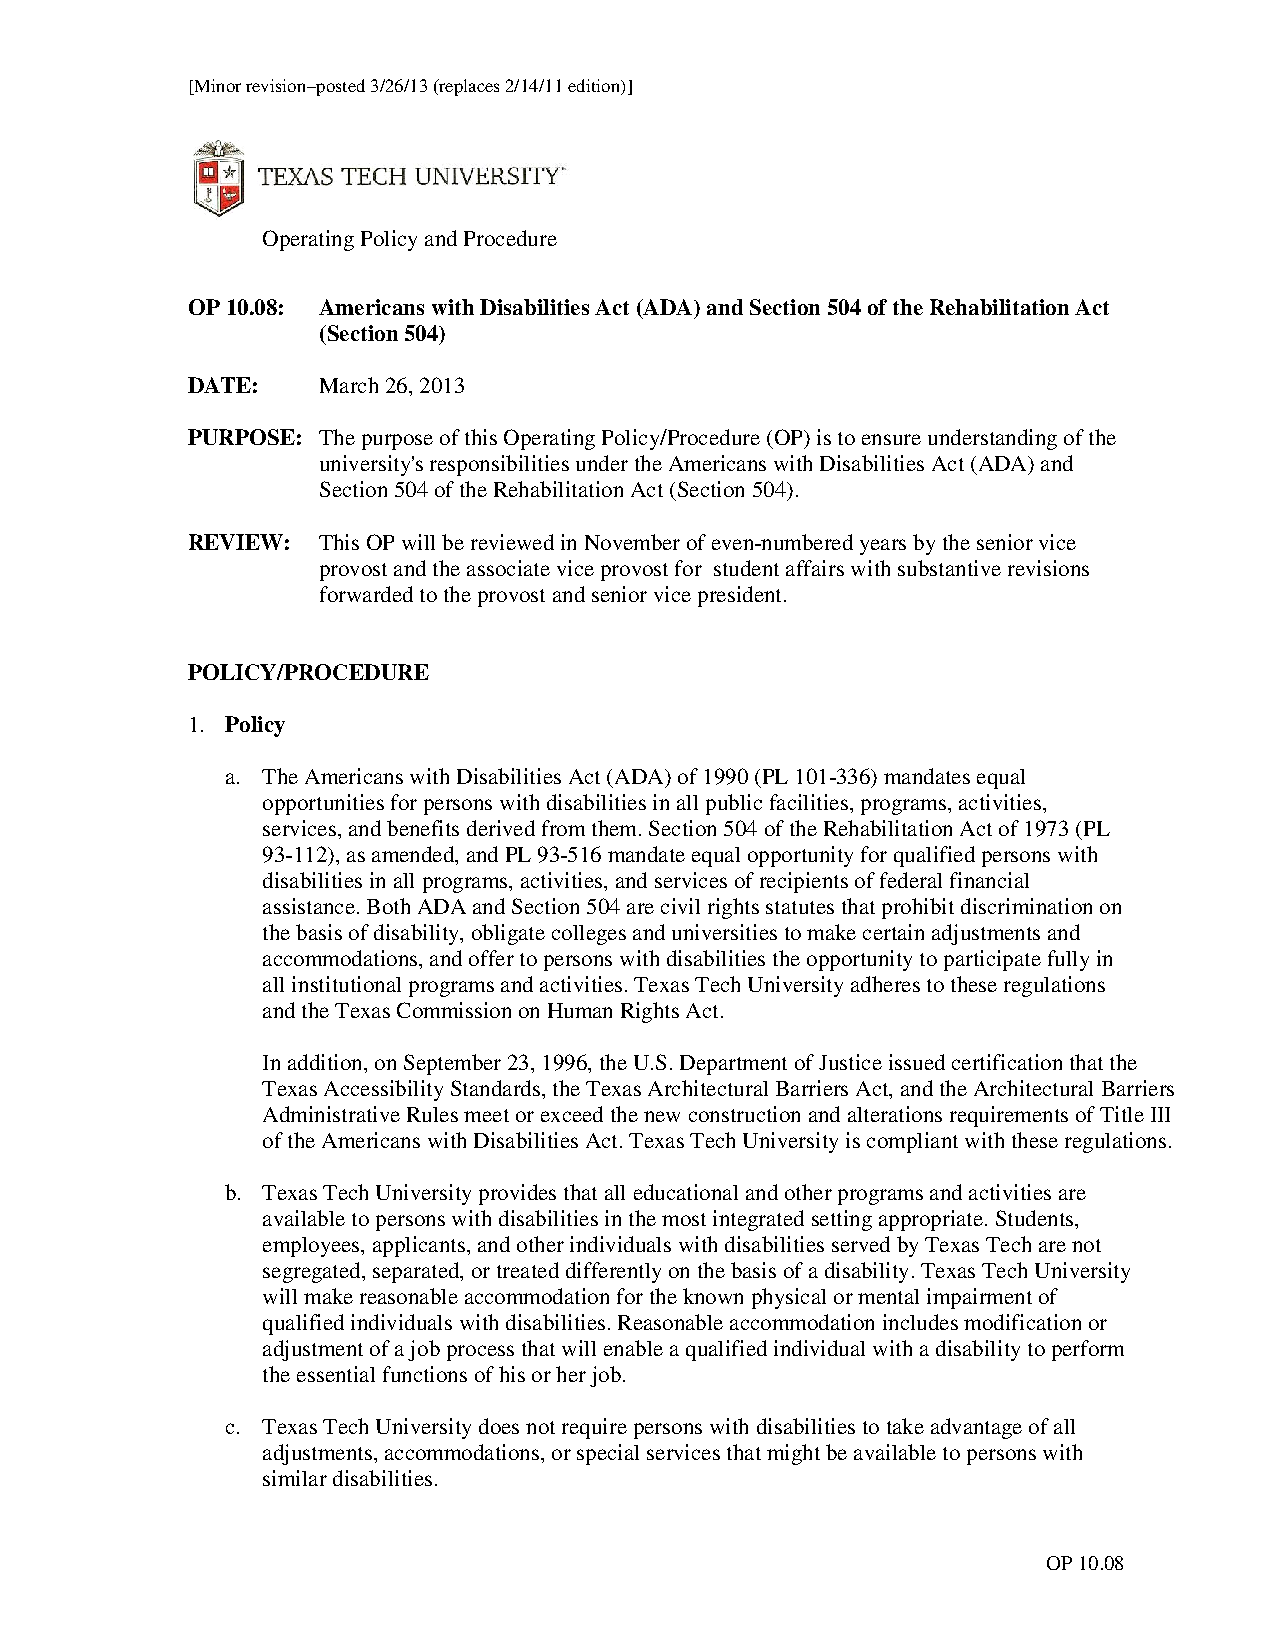
\includepdf[pages=-]{./OP10-08.pdf}

\section*{Required Syllabus Statements}
\url{https://www.depts.ttu.edu/tlpdc/RequiredSyllabusStatements.php}
\subsection*{ADA STATEMENT:}
Any student who, because of a disability, may require special arrangements in order to meet the course requirements should contact the instructor as soon as possible to make any necessary arrangements. Students should present appropriate verification from Student Disability Services during the instructor's office hours. Please note: instructors are not allowed to provide classroom accommodations to a student until appropriate verification from Student Disability Services has been provided. For additional information, please contact Student Disability Services in Weeks Hall or call 806-742-2405.

\subsection*{ACADEMIC INTEGRITY STATEMENT:}
Academic integrity is taking responsibility for one's own class and/or course work, being individually accountable, and demonstrating intellectual honesty and ethical behavior. Academic integrity is a personal choice to abide by the standards of intellectual honesty and responsibility. Because education is a shared effort to achieve learning through the exchange of ideas, students, faculty, and staff have the collective responsibility to build mutual trust and respect. Ethical behavior and independent thought are essential for the highest level of academic achievement, which then must be measured. Academic achievement includes scholarship, teaching, and learning, all of which are shared endeavors. Grades are a device used to quantify the successful accumulation of knowledge through learning. Adhering to the standards of academic integrity ensures grades are earned honestly. Academic integrity is the foundation upon which students, faculty, and staff build their educational and professional careers. [Texas Tech University (“University”) Quality Enhancement Plan, Academic Integrity Task Force, 2010].


\subsection*{RELIGIOUS HOLY DAY STATEMENT:}
"Religious holy day" means a holy day observed by a religion whose places of worship are exempt from property taxation under Texas Tax Code §11.20. A student who intends to observe a religious holy day should make that intention known in writing to the instructor prior to the absence. A student who is absent from classes for the observance of a religious holy day shall be allowed to take an examination or complete an assignment scheduled for that day within a reasonable time after the absence. A student who is excused under section 2 may not be penalized for the absence; however, the instructor may respond appropriately if the student fails to complete the assignment satisfactorily.

\subsection*{STATEMENT OF ACCOMMODATION FOR PREGNANT STUDENTS:}
To support the academic success of pregnant and parenting students and students with pregnancy related conditions, the University offers reasonable modifications based on the student's particular needs. Any student who is pregnant or parenting a child up to age 18 or has conditions related to pregnancy may contact Alex Faris, the Texas Tech University designated Pregnancy and Parenting Liaison, to discuss support available through the University. The Liaison can be reached by emailing alfaris@ttu.edu. Should a student communicate with the instructor that they are pregnant or have a pregnancy related condition or may need additional resources related to pregnancy or parenting, the instructor will communicate that student's information to the Title IX Coordinator, who will work with the student and others, as needed, to ensure equal access to the University's education program or activity. 

For more information regarding supportive measures, please contact pregnancy \& parenting liaison Alex Faris (alfaris@ttu.edu : 806.834.3420) or visit \url{https://www.depts.ttu.edu/titleix/PregnacnyandParenting/index.php}. 
You can also visit \url{https://www.depts.ttu.edu/titleix/PregnacnyandParenting/index.php} to submit a request to Alex Faris for assistance.

\section*{Recomended/Optional Syllabus Statements}
\url{https://www.depts.ttu.edu/tlpdc/RecommendedSyllabusStatements.php}

\subsection*{DISCRIMINATION, HARASSMENT, AND SEXUAL VIOLENCE STATEMENT:}

Texas Tech University is committed to providing and strengthening an educational, working, and living environment where students, faculty, staff, and visitors are free from gender and/or sex discrimination of any kind. Sexual assault, discrimination, harassment, and other Title IX violations are not tolerated by the University. Report any incidents to the Office for Student Rights \& Resolution, (806)-742-SAFE (7233) or file a report online at \url{titleix.ttu.edu/students}. Faculty and staff members at TTU are committed to connecting you to resources on campus. Some of these available resources are: 
\begin{itemize}
\item TTU Student Counseling Center, 806- 742-3674, \url{https://www.depts.ttu.edu/scc/}(Provides confidential support on campus.) 
\item TTU 24-hour Crisis Helpline, 806-742-5555, (Assists students who are experiencing a mental health or interpersonal violence crisis. If you call the helpline, you will speak with a mental health counselor.) 
\item Voice of Hope Lubbock Rape Crisis Center, 806-763-7273, \url{voiceofhopelubbock.org} (24-hour hotline that provides support for survivors of sexual violence.) 
\item The Risk, Intervention, Safety and Education (RISE) Office, 806-742-2110, \url{https://www.depts.ttu.edu/rise/} (Provides a range of resources and support options focused on prevention education and student wellness.) 
\item Texas Tech Police Department, 806-742-3931, \url{http://www.depts.ttu.edu/ttpd/} (To report criminal activity that occurs on or near Texas Tech campus.)
\end{itemize}
 
\subsection*{RECOVERY SERVICES STATEMENT:}

The Center for Students in Addiction Recovery offers students in recovery a nurturing and supportive community. The Center provides students in recovery with an abstinence-based program where students can flourish in recovery as they attain educational goals, including advanced degrees. The services provided through the CSAR increases the continuum of care for students in recovery, enhancing the quality of life for students in recovery at Texas Tech University. The CSAR supports students in recovery from alcohol, drugs, and behavioral addictions. By providing recovery support through relationships with staff, academic advising, scholarships / fellowships, recovery housing, study abroad opportunities, and more, students can flourish in recovery and in life.

 
\subsection*{CIVILITY IN THE CLASSROOM STATEMENT:}

Texas Tech University is a community of faculty, students, and staff that enjoys an expectation of cooperation, professionalism, and civility during the conduct of all forms of university business, including the conduct of student–student and student–faculty interactions in and out of the classroom. Further, the classroom is a setting in which an exchange of ideas and creative thinking should be encouraged and where intellectual growth and development are fostered. Students who disrupt this classroom mission by rude, sarcastic, threatening, abusive or obscene language and/or behavior will be subject to appropriate sanctions according to university policy. Likewise, faculty members are expected to maintain the highest standards of professionalism in all interactions with all constituents of the university (\url{www.depts.ttu.edu/ethics/matadorchallenge/ethicalprinciples.php}).

 
\subsection*{PLAGIARISM STATEMENT:}

Texas Tech University expects students to “understand the principles of academic integrity and abide by them in all class and/or course work at the University” (OP 34.12.5). Plagiarism is a form of academic misconduct that involves (1) the representation of words, ideas, illustrations, structure, computer code, other expression, or media of another as one's own and/or failing to properly cite direct, paraphrased, or summarized materials; or (2) self-plagiarism, which involves the submission of the same academic work more than once without the prior permission of the instructor and/or failure to correctly cite previous work written by the same student. This video, retrieved from the University of Kansas Libraries website, provides an example of a plagiarism definition as well as examples of plagiarism and how to avoid it. Please review Section B of the TTU Student Handbook for more information related to other forms of academic misconduct, and contact your instructor if you have questions about plagiarism or other academic concerns in your courses. To learn more about the importance of academic integrity and practical tips for avoiding plagiarism, explore the resources provided by the TTU Library and the School of Law.

 
\subsection*{STUDENT SUPPORT STATEMENT:}

The Office of Campus Access and Engagement works across Texas Tech University to foster, affirm, celebrate, engage, and strengthen all student communities. For more information about services, opportunities for participation, and ways in which Texas Tech can support your success in college, please contact (806) 742-7025.

 
\subsection*{STATEMENT ABOUT FOOD INSECURITY:}

Any student who faces challenges securing their food or housing and believes this may affect their performance in the course is urged to contact the Dean of Students for support. Furthermore, please notify the professor if you are comfortable in doing so. Raider Red's Food Pantry (located in Doak 117) supplies personal care items and a selection of nonperishable food to students. The Raider Relief Advocacy and Resource Center (RR- ARC) is a centralized hub of resources and support for students facing hardships with their basic needs. Through a comprehensive network of campus and community partnerships, we strive to alleviate the burden of financial, physical, and emotional hardships and promote the well-being and academic success of all students. Please fill out our form to get connected: \url{https://www.depts.ttu.edu/raiderrelief/}.

 
\subsection*{RISK ASSOCIATED WITH THE USE OF LIVESTOCK/HORSES STATEMENT:}

Working with livestock is inherently risky. Animals are capable of injuring people, especially when they are in the fight or flight mode in response to stress or unfamiliar situations. The instructor will work to provide students with the ability to manage horses or livestock with minimal stress, thus decreasing the risk of injury to people and animals. It is imperative that students follow instructions and communicate any discomfort with assigned activities. Please see link for additional information on animal-borne diseases: \url{https://www.depts.ttu.edu/iacuc/Zoonoses_Guidelines.php}

 
\subsection*{RISK ASSOCIATED WITH THE USE OF COMPANION ANIMALS STATEMENT:}

Working with companion animals can be inherently risky. Dogs and cats are capable of injuring people, especially when they are fearful or in unfamiliar situations. The instructor will work to provide students with the ability to handle dogs and cats with minimal stress, thus decreasing the risk of injury to people and animals. It is imperative that students follow instructions and communicate any discomfort with assigned activities. Please see link for additional information on animal-borne diseases: \url{https://www.depts.ttu.edu/iacuc/Zoonoses_Guidelines.php}

 
\subsection*{RISK ASSOCIATED WITH THE USE OF WILDLIFE STATEMENT:}

Working with wildlife is inherently risky. Some wildlife species are capable of injuring people and/or spreading zoonotic diseases. The instructor will work to provide students with the ability to handle wildlife species with minimal stress, thus decreasing the risk of injury to people and animals. It is imperative that students follow instructions and communicate any discomfort with assigned activities. Please see link for additional information on animal-borne diseases: \url{https://www.depts.ttu.edu/iacuc/Zoonoses_Guidelines.php}

\section*{AI Use Syllabus Statements:}
\url{https://www.depts.ttu.edu/tlpdc/AI_Resources/AI-Use-is-Encouraged.pdf}
\subsection*{AI Use is encouraged and allowed in your course:}
You may use generative artificial intelligence (AI) tools (such as ChatGPT) in this class, as doing so aligns with our course learning goals. Your use of AI tools must be properly documented and cited. You are responsible for ensuring the information you submit based on an AI query does not contain misinformation, unethical content, or violate intellectual property laws. Submission of AI-generated content as your own work is a violation of academic integrity and may result in referral to the Office of Student Conduct. Please contact your instructor if you have questions regarding this course policy.\footnote{AI responses are often incorrect; be sure the response makes sense, is correct, and grammatically edited.  AI responses must be disclosed in your work.}

\section*{ADDITIONAL COURSE SPECIFIC POLICIES:}
\subsection*{Cellphones/Pagers: }
Please set your personal communication devices to silent ring or off during class. Do not take calls in class. Disturbance during class time is not acceptable.
\subsection*{Prerequisites:} 
Mastery of material from CE 3305 or equivalent is expected.
\subsection*{Attendance:} Roll will be taken to determine attendance for class participation.  Please let the instructor know in advance if you must miss a class for a legitimate reason\footnote{Legitimate reasons include: Academically-related extracurricular activities (ASCE, AGU, etc.); Illness with documentation; Federal Family Leave Act Policies; Orders to activate (Military, Peace Officer, Public Health, etc.).  Show me some kind of documentation for such absences.}. 

\section*{Evaluation Instruments and Grading}
Student performance will be evaluated using attendance (coming to class), homework, project reports, and examinations.   The examinations will derive much of their content from the exercises.  %At the end of the semester students are to turn in a portfolio of all graded work.  The portfolio should be comprised of photocopies of exercise materials, and exams 1 and 2.  The project report should be submitted under separate cover.  The portfolio should be bound using a binder clip.  The portfolio will not be returned.  

%\subsection*{Article Reviews:} 
%Several article reviews are assigned; part of professional development is reading and interpreting professional literature.  Due dates for these reviews are shown in Table \ref{tab:fall2014schedule}.  These reviews are shown as \texttt{R-\#}.

\subsection*{Homework:} 
Homework assignments are distributed and collected using Blackboard.  Check frequently as the semester proceedes.  Due dates are on Blackboard.  
These exercises are scored (usually) on a 100 point criteria\footnote{Legibility, correct method, and correct answer are components of the criteria.   
The grader will not diagnose sources of arithmetic or algebra errors unless the errors are obvious.  
Once solutions are presented in class and/or posted on the server, the maximum point allowance is substantially reduced}.

\subsection*{Semester Project:}  
A semester project comprised of various components developed during the course is to be completed by teams of 3-5 people.  .  
The project is a hydrologic analysis of a watershed, that uses methods described during the semester. 
A presentation and final report are required (all team members will submit a final report).

\subsection*{Exams:} Three in-class examinations are scheduled, they will be of approximately equal difficulty.  
\begin{enumerate}
\item Examinations are open notes.
\item Examinations are comprehensive, even though the main focus will be the materials discussed prior to the examination.
\item Full credit for problems will only be given if all computations are documented.
\end{enumerate}

\section*{Grading:} Final grades are determined based on performance during the semester.  Letter grades will be assigned using University standards.  The \textbf{approximate} weighting of graded material in determining the final grade is as follows\footnote{Graded materials with fewer than 100 points will have raw scores reported and will be normalized to 100 points for calculating the final grade.}:
% Requires the booktabs if the memoir class is not being used
\begin{table}[h!]
   \centering
   \begin{tabular}{l l}
Item & Percent of Grade \\
\hline
\hline
Attendance & 10\% \\
Exercises & 20\% \\
Project Report & 10\% \\
Project Presentation & 10\% \\
Examinations & 50\% \\
\hline
\end{tabular}
\end{table}

\textbf{Cheating:} Dont!

%%%%%%%%%SCHEDULE GOES HERE %%%%%%%%%
%%%%%%%%% Use Comment to Maintain History %%%%%
\clearpage
\section*{Schedule}
\begin{table}[ht!]
   \centering
   \caption{Fall 2024 Course Schedule}
   \begin{tabular}{p{0.5in}p{3.0in}p{3.0in}} 
   ~ & ~ & ~  \\
\hline
DATE & TOPIC & READINGS  \\
\hline
\texttt{22AUG24} & Introduction & Server Notes  \\ %0
\texttt{27AUG24} & Specialized Software & RSG(pp.781-802) \\ %1 
\texttt{29AUG24} & Hydrologic Cycle  & RSG(pp.39-46);CMM(pp.1-12)\\ %2 water budget(s) ES-1 (Water Budget)
\texttt{~3SEP24} & Hydrologic Data Sources & RSG(pp.273-326);CMM(pp.175-201)\\ %3 streamflow measurement, precipitation measurement, online archives
\texttt{~5SEP24} & Watersheds and GIS &  \\ %4 watershed definitions and delineation, metrics of interest ES-2 (Watershed Delineation; Web Soil SUrvey)
\texttt{10SEP24} & Probability Estimation Modeling &  RSG(pp.423-442);CMM(pp.350-380)\\ %5
\texttt{12SEP24} & Streamflow and Hydrographs & RSG(pp.93-123;);CMM(pp.127-175)\\ %6 ES-3 (Precipitation, Runoff Data Plots; Oklahoma Empirical Return Period)
\texttt{17SEP24} & WCOE Job Fair (Civil Engineering)   &   \\ %7
\texttt{19SEP24} & Floods and Flood Frequency Analysis & RSG(pp.442-469);CMM(pp.380-416) \\ %8 ES-4 (FloodFrequency B17C)
\texttt{24SEP24} & Precipitation, Hyetographs, Design Storms &  RSG(pp.46-59);CMM(pp.444-493) \\  %9 NOAA Atlas 14, PFDS, Create design storm
\texttt{26SEP24} & \textbf{Exam 1} &  \\ % XBS Watershed Delineation; Flood Frequency; Water Budget; 
\texttt{~1OCT24} & Evaporation and Infiltration Losses & RSG(pp.65-88; 93-111);CMM(pp.99-127) \\ %10
\texttt{~3OCT24} & Rainfall-Runoff Modeling, NRCS Runoff Generation & RSG(pp.93-123) \\ %11
\texttt{~8OCT24} & Rational and Modified Rational Method & RSG(pp.711-734) \\  %12  
\texttt{10OCT24} & Unit Hydrographs & RSG(pp.350-361);CMM(pp.201-221)\\ %13
\texttt{15OCT24} & Synthetic Unit Hydrographs & RSG(pp.362-371);CMM(pp.221-242) \\ %14
\texttt{17OCT24} & HEC-HMS  & SN \\ %15
\texttt{22OCT24} & Reservoir Routing &RSG(pp.477-492;503-506);CMM(pp.242-252)  \\ %16
\texttt{24OCT24} & Catchment Routing &RSG(pp.497-502);CMM(pp.257-272;302-310)\\ %17
\texttt{29OCT24} & Reservoir Storage and Discharge & RSG(pp.545-575)\\ %18
\texttt{31OCT24} & \textbf{Exam 2} & \\ %YBS Rational; Modified Rational; UH Analysis
\texttt{~5NOV24} & H\&H - Storm Sewer Sizing &RSG(pp.711-734);CMM(pp.493-517)  \\ %19
\texttt{~7NOV24} & H\&H Design - Culvert Sizing & RSG(pp.761-770);CMM(pp.XXX-XXX)  \\ %20
\texttt{12NOV24} & Groundwater Hydrology & RSG(pp.127-135)  \\ %21 
%%%%%%%%%%%%%%%%%%%%%%%%%%%%%%%%%%%%%%%%%%%%%%%%%%%%%%%%%%%%
\texttt{14NOV24} & Groundwater Flow Mechanics & RSG(pp.136-154) \\ %22
\texttt{19NOV24} & Well Hydraulics & RSG(pp.167-187) \\ %23
\texttt{21NOV24} & Pumping Tests & RSG(pp.187-215) \\ %24
\texttt{26NOV24} & Team Presentations &  Teams 1-6\\ %25
\texttt{28NOV24} & Thanksgiving Holiday &    \\ %26
\texttt{~3DEC24} & Team Presentations & Teams 7-12 \\ %27
\texttt{~6DEC24} & \textbf{Exam 3} & 07:30-10:00 \\ %ZBS Storm Sewer; Routing ; HEC-HMS; Pumping Test; Wellfield
\hline
   \end{tabular}
   \label{tab:schedule}
\end{table}

%RSG = \cite{Gupta2017};
%CMM = \cite{CMM1988}; 
%LS = \cite{Dooge1973} ;
%SN = \cite{Cleveland2024};

\clearpage



\begin{thebibliography}{}

\bibitem[Chow and others(1988)]{CMM1988}
Chow, V.T., Maidment, D.R., Mays, L.W., 1988, Applied Hydrology: New York,
McGraw-Hill.

\bibitem[Dooge(1973)]{Dooge1973}
Dooge, J.C.I. 1973.  Linear Theory of Hydrologic Systems. ARS Technical Bulletin No. 1468.  US Department of Agriculture, Washington, D.C.

\bibitem[McCuen and others(2002)]{McCuen2002}
Richard H. McCuen, Peggy A. Johnson, Robert M. Ragan, 2002.  Highway Hydrology; Hydraulic Design Series Number 2, Second Edition.  
Federal Highway Administration, National Highway Institute, 4600 North Fairfax Drive, Suite 800, Arlington, Virginia 22203.  424p.

\bibitem[Gupta(2017)]{Gupta2017}
Gupta, R.S. 2017. Hydrology and Hydraulic Systems 4th ed. Waveland Press, Inc. ISBN 978-1-4786-3091-3 888p.

\bibitem[Cleveland(2024)]{Cleveland2024}
Cleveland, T. G. 2024. Engineering Hydrology Instructor's Notes and Selected Readings to accompany CE-3354, Department of Civil, Environmental, and Construction Engineering, Whitacre College of Engineering. \url{http://54.243.252.9/ce-3354-webroot/}

\end{thebibliography}

\end{document}  